\section{Introduction}
As a promising solution in the clean energy, photovoltaic (PV) systems have drawn great attention recently. An accurate PV system model is the kernel in the PV system optimization. Furthermore, a fast and accurate model is more attractive when real time applications, such as to capture the PV system characteristics with ever-changing shadings \cite{koutroulis2001development, xiao2004modified}, are required.

A PV system model needs to consider mismatches across solar cells in PV systems. Mismatches have to be considered for two reasons. First, a PV system has numerous solar cells - a PV system consists of thousands of PV modules, and each PV module consists of cascaded and paralleled solar cells. Thus, solar cell mismatches are inevitable. Second, PV systems are vulnerable to mismatches. Mismatches, such as temperature variations, non-uniform cell aging, and non-uniform shading across the cells, can cause power losses and solar cell damages \cite{herrmann1997hot}. The non-uniform shading is also known as the Shading Effects \cite{shading1, sullivan1965shadow}. Shading Effects lead to the largest output power reduction and cell damage \cite{shading1}. Furthermore, the shading on PV module is always changing. It needs a fast PV system model.

The bypass diode is another essential part in a PV module, and has to be modeled accurate in a PV module model. Bypass diodes are connected in parallel to solar cells. Figure \ref{fig:colexample} shows a solar cell chain with $3$ bypass diodes. Bypass diodes have been proven to be an effective solution to compensate for consequences cause by mismatches \cite{bp1}.

%insert figure 1
\begin{figure}[tb]
    \centering
    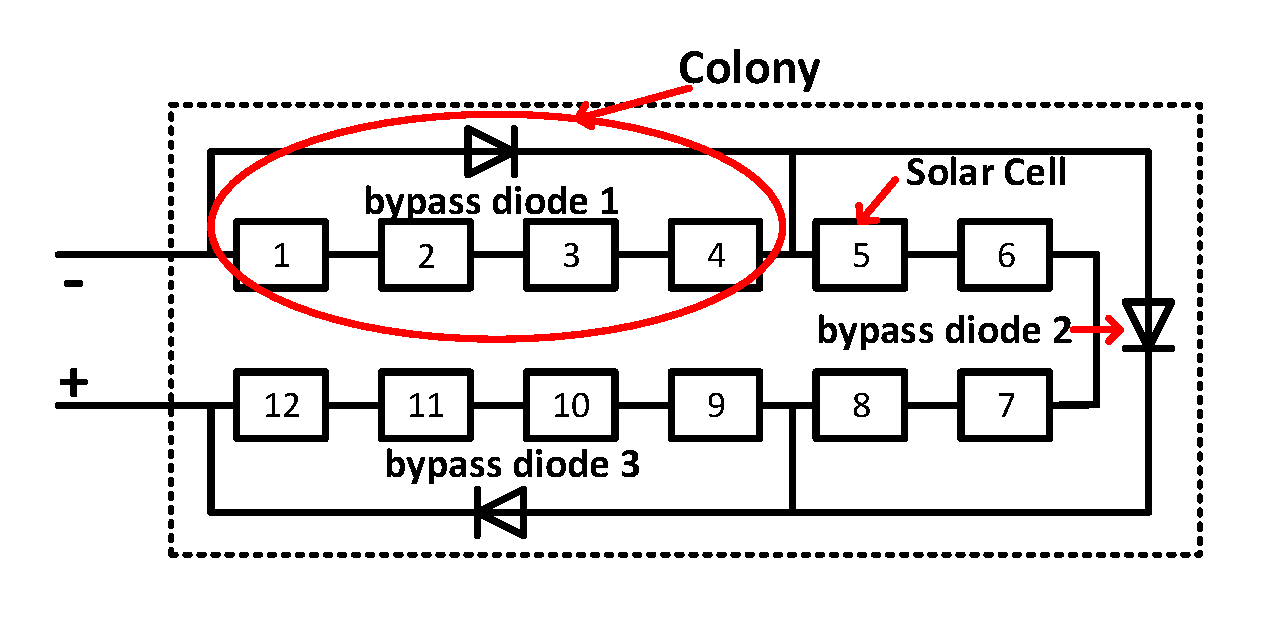
\includegraphics[width=1\columnwidth]{figs/colony_example_new.pdf}
    \caption{A PV module with 1 solar cell chain, which consists of 12 solar cells and 3 colonies.}
    \label{fig:colexample}
\end{figure}

A PV system��s model is based on PV module models. The existing PV module models are equivalent circuit models \cite{oneD1, oneD3}. Generally, a solar cell is modeled as a circuit, with a current source, diodes and resistors. A well-accepted solar cell model is shown in Figure \ref{fig:oneD}. It is referred to as the \textit{One-Diode model} in this paper. A PV module model is then modeled by cascaded and paralleled One-Diode solar cell models, along with the bypass diodes according to the PV module��s configuration. Each One-Diode solar cell has its own parameters to model mismatches. This PV module model offers great accuracy. We refer this model as the \textit{Ground Truth (GT)} model throughout this paper. An example is as in Figure \ref{fig:colexample}. It is a PV module with a single solar cell chain that consists of $12$ solar cells and $3$ bypass diodes. Therefore, its GT model has $12$ One-Diode models and $3$ diode models. The major drawback of the GT model is its computational time. The GT model��s complexity is proportional to the number of solar cells. Consequently, the reduction of PV module model��s complexity is appealing.

\begin{figure}[tb]
    \centering
    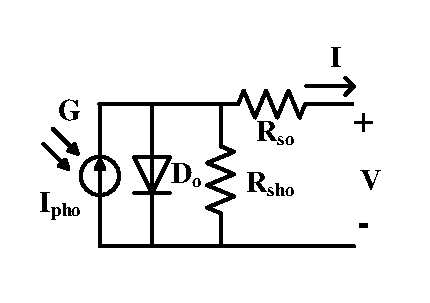
\includegraphics[width=0.7\columnwidth]{figs/one_diode_diagram.pdf}
    \caption{The One-Diode model of a solar cell.}
    \label{fig:oneD}
\end{figure}

In this paper, we propose two PV module models to solve the above problem. The first model is call the \textit{Colony-Wise (CW)} model. A \textit{colony} is defined as a bypass diode plus all its paralleled solar cells, as shown in the circle in Figure \ref{fig:colexample}. The number of colonies inside a PV module equals its quantity of bypass diodes. Solar cells inside of each colony are lumped into at most two \textit{macro cells}. The macro cell is modeled as the One-Diode model. Compared with the GT model, the CW model remains high accuracy, while its complexity is only proportional to the number of bypass diodes in a PV module.

We proposed a second \textit{N-Colony (NC)} model to further reduce the complexity. The N-Colony model models a PV module with at most N colonies, where N is the number of bypass diodes in a module��s cascaded solar cell chain. All solar cells inside each colony are only modeled by one \textit{super cell}. This super cell is again modeled by the One-Diode model. The NC model achieves constant computational complexity with acceptable accuracy.

Our major contribution is that these two models can model PV module of various configurations and with shading effects accurately and efficiently.

The rest of this paper is organized as follows. Section II presents the One-Diode solar cell model, and how to represent shading effects and PV module configurations. These are the preliminaries of our proposed PV module models. Section III and Section IV introduce and validate the Colony-Wise model and the N-Colony Model respectively. Section V compares these two new models with the Ground Truth model. Finally, Section VI concludes the paper.

